\documentclass{article}
\usepackage{tikz}
\usetikzlibrary{arrows.meta}

\begin{document}

\begin{figure}[h]
    \centering
    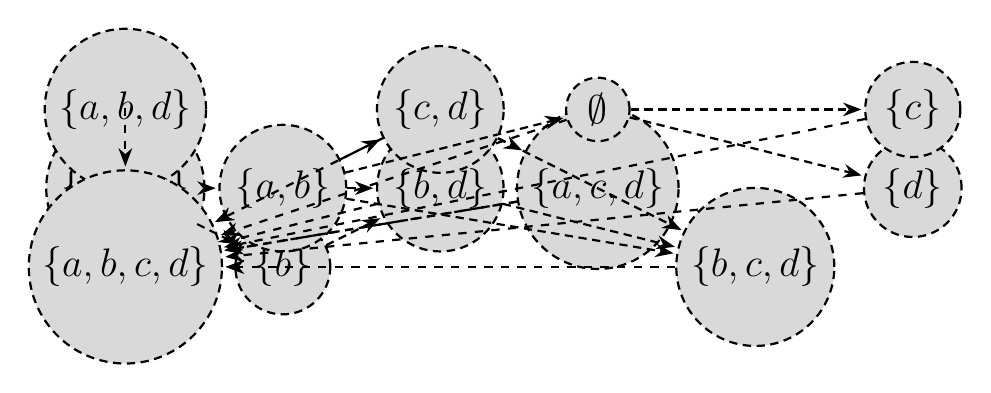
\begin{tikzpicture}[->,>=Stealth,dash pattern=on 3pt off 2pt,shorten >=1pt,auto,node distance=2cm,
    thick,main node/.style={circle,fill=gray!30,draw,font=\sffamily\Large\bfseries}]

        % Nodes
        \node[main node] (1) at (-5,0) {$\{a,b,c\}$};
        \node[main node] (2) at (-3,-1) {$\{b\}$};
        \node[main node] (3) at (-3,0) {$\{a,b\}$};
        \node[main node] (4) at (-1,0) {$\{b,d\}$};
        \node[main node] (5) at (-1,1) {$\{c,d\}$};
        \node[main node] (6) at (1,0) {$\{a,c,d\}$};
        \node[main node] (7) at (1,1) {$\emptyset$};
        \node[main node] (8) at (3,-1) {$\{b,c,d\}$};
        \node[main node] (9) at (5,0) {$\{d\}$};
        \node[main node] (10) at (5,1) {$\{c\}$};
        \node[main node] (11) at (-5,1) {$\{a,b,d\}$};
        \node[main node] (12) at (-5,-1) {$\{a,b,c,d\}$};

        % Edges
        \path[every node/.style={font=\sffamily\small}]
            (1) edge node [left] {} (2)
            (1) edge node [left] {} (3)
            (3) edge node [right] {} (4)
            (3) edge node [right] {} (5)
            (5) edge node [right] {} (6)
            (3) edge node [right] {} (7)
            (6) edge node [right] {} (8)
            (5) edge node [above] {} (8)
            (7) edge node [above] {} (9)
            (7) edge node [above] {} (10)
            (2) edge node [right] {} (4)
            (3) edge node [right] {} (8)
            (4) edge node [right] {} (8)
            (6) edge node [right] {} (12)
            (1) edge[dashed] node [left] {} (12)
            (2) edge[dashed] node [left] {} (12)
            (3) edge[dashed] node [left] {} (12)
            (4) edge[dashed] node [left] {} (12)
            (5) edge[dashed] node [left] {} (12)
            (6) edge[dashed] node [left] {} (12)
            (7) edge[dashed] node [left] {} (12)
            (8) edge[dashed] node [left] {} (12)
            (9) edge[dashed] node [left] {} (12)
            (10) edge[dashed] node [left] {} (12);

    \end{tikzpicture}
    \caption{Transition graph $\Gamma_1$ of temporal program $\Pi_1$. The nodes that belong to some solution of length $4$ have a gray background. The transitions of those solutions are represented by normal arrows, while the other arrows are dashed.}
    \label{fig:trans_graph}
\end{figure}

\end{document}